\chapter{Introdução}

%As citações são feitas usando o comando~\texttt{\textbackslash cite}. Para usar colchetes nas citações, use o comando \texttt{\textbackslash citeC}. Exemplo


\section{Contextualização e Definição do Problema}
	\subsection{Efeito  de ambientização: \textit{Reverb}}
	\label{aplicabilidade}
		
		Numa sala, ou em qualquer ambiente acústico, existe um caminho direto pelo qual uma fonte de áudio qualquer pode ser ouvida, no entanto, as respectivas ondas sonoras também podem fluir em caminhos mais longos devido a, por exemplo, reflexão das paredes, do teto, de objetos, antes delas chegarem ao receptor.
		
		A energia envolvida som dessas reflexões, as quais viajam essas distâncias maiores do que o som emitido no caminho direto, são parcialmente absorvidas pelas superfícies, logo elas chegam ao receptor com um som mais "fraco" que o som direto.
		
		Essas amostras de som atrasadas e atenuadas ocorridas no evento da emissão do som original é o que denominamos de \textbf{reverbaração}.
		
		\begin{figure}[!ht]
			\centering
			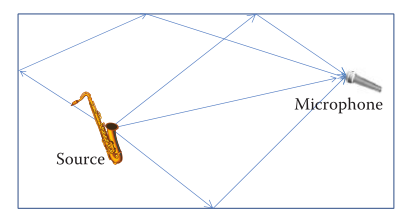
\includegraphics[scale=0.5]{./figuras/reverb01.png}
			\caption{Ilustração do efeito de Reverberação.}
			\label{reverb01}
		\end{figure}
		
		Muito embora possa parecer ao primeiro momento, o efeito de reverberação é muito mais que uma série de ecos. Um eco, por exemplo, pode ser entendido um resultado de uma distinção, atraso de versões de um som, o qual você pode ouvir com um atraso no mínimo de 40 milissegundos. Já a reverberação de uma sala vazia, por exemplo, há muitas e muitas reflexões, e as primeiras delas que chegam ao receptor são muito mais curtas que termos de tempo de duração. Logo essas reflexões não são tão percebidas ou distinguidas do som da fonte diretamente. Em vez disso, nós percebemos apenas o efeito da combinação de todas essas reflexões.
		
		\begin{figure}[!ht]
			\centering
			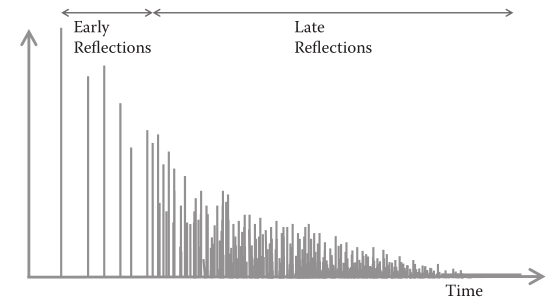
\includegraphics[scale=0.5]{./figuras/reverb02.png}
			\caption{Resposta de um Impulso de uma sala pequena.}
			\label{reverb02}
		\end{figure}
		
		Nesse sentido, podemos também considerar que a reverberação do som é mais do que um simples dispositivo de \textit{delay} com retorno. No \textit{reverb} a taxa em que as reflexões chegarão muda ao longo do tempo, em oposição de termos apenas que simular reflexões que tenham um intervalo fixo entre elas. Essas reflexões são relacionadas a posição do som que o receptor está na sala, ao tipo de construção da sala (oval, retangular), tamanho e material das paredes. 
		
		
	\subsection{Tipos de Reverb}
	
		Efeitos de \textit{reverb} são alcançados pela utilização de uma série complexa de \textit{delays} de um mesmo sinal que diminuem em amplitude e clareza de modo a simular o comportamento acústico de um espaço real. Falando sob o aspecto musical e industrial de equipamentos que realizam o processamento e simulação de efeitos de repetição (tal como o reverb, delay) termos no mercado diversos tipos de \textit{reverb`s}, os quais possuem diferentes aplicações que veremos a seguir:
		
		\begin{itemize}
			\item \textbf{Spring} ("Reverb-de-mola") - O efeito de reverberação com mola é um método que foi primeiramente proposto por \textit{Hammond} em 1940s. O reverb de mola foi criado naturalmente, por um sistema mecânico, o qual usa um transdutor e um captador nas extremidades de uma mola, para criar e capturar vibrações dentro dela. Muitos amplificadores de guitarra incluem esse tipo de reverberação dentro de seus projetos. Existem ainda muitos pedais de reverb que oferecem esse efeito emulado digitalmente e apenas algumas companhias, por questões de custo de construção, também lançaram produtos com um sistema real de reverb de molas.
			
			\begin{figure}[!h]
				\centering
				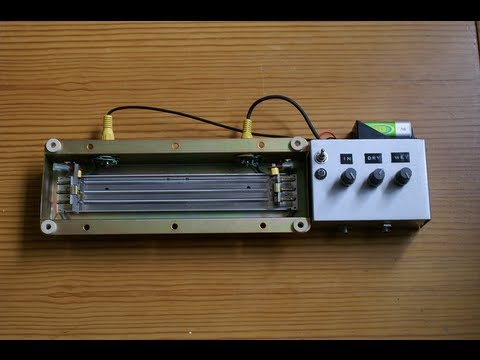
\includegraphics[scale=0.3]{./figuras/spring-reverb.jpg}
				\caption{Câmara de reverb de mola de um amplificador}
				\label{spring-reverb}
			\end{figure}
			
			\item \textbf{Room} ("Reverb-sala") - Este tipo de reverb é usado para simular um som natural de uma sala acústica, geralmente vazia, que tem um tamanho geralmente pequeno. Esses reverbs usualmente possuem reflexões curtas que desaparecem rapidamente com o tempo. 
			
			\item \textbf{Hall} ("Reverb-palco") - Reverb's dessa categoria são usados para simular um tipo de reverberação encontrado num grande teatro ou até mesmo catedrais ou igrejas. Eles "soam" geralmente mais fortes do que um \textit{room reverb} por conta da quantidade de reflexões serem significativamente maiores e mais longas. Pode ser encontrado a variação de hall reverbs como "\textit{cathedral}".
			
			\item \textbf{Plate} ("Reverb-de-placas") - Um plate reverb é definitivamente o efeito que exige uma grande logística a ser empregada. Uma grande máquina conforme mostrado na figura () a qual fornece o áudio dentro de grandes "placas" penduradas de metal que produzem um som de reverb que é mais definido do que o efeito do hall-reverb enquanto ainda é capaz de produzir longos decaimentos no tempo.
			
			\begin{figure}[!h]
				\centering
				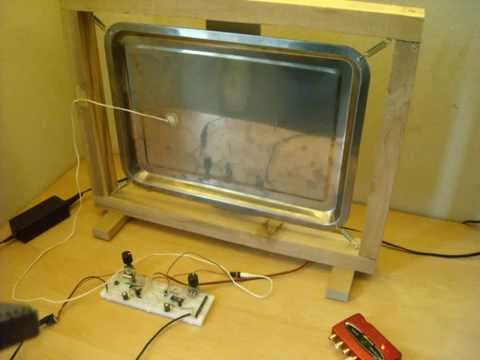
\includegraphics[scale=0.3]{./figuras/plate-reverb.jpg}
				\caption{Pequeno protótipo de um reverb de placas.}
			\end{figure}
			
			\item \textbf{Pitch-Shifter Reverb} aka \textbf{Shimmer} - Bem esse efeito de reverb será o foco de desenvolvimento desse trabalho. O shimmer tem se tornado bem comum entre pedais de guitarra principalmente nesses últimos anos. A grosso modo, esses reverbs adicionam componentes harmônicos do som original para dar a sensação de ambiência e harmonia e simulam a reverberação desses sons mais agudos na "cauda" (no final do reverb).
			
			Este som tem características bem peculiares, as quais geralmente as pessoas associam a um som de orquestra angelical ou sintetizadores de teclado, dando uma intensa ambiência e atmosfera no som.
			
			Diferente dos demais reverbs, o Shimmer é um efeito eminentemente sintetizado, ou seja, produzido digitalmente por meio de algoritmos embarcados em DSP`s e comercializados como equipamentos de produção digital.
			
		\end{itemize}
	
	\subsection{Pitch Shifting}
	\label{introd-pitch-shift}
	
		\subsubsection{Conceitos Inicias}
		
			Entre os efeitos digitais de áudio (especialmente os realizados em tempo real), esse é um dos que exige algoritmos mais sofisticados, e até recentemente, os resultados não eram convincentes. 
			
			A primeira consideração a ser feita sobre esse assunto seria entender o que é um \textit{pitch shifting}. A melhor definição para o termo "pitch"de um som seria o conjunto de frequências de que o som é formado. A melhor maneira de entender esta definição é olhar por exemplo um coral. Nele há tanto mulheres quanto homens cantando mas as mulheres tem um "alcance"/pitch mais alto que o homem. A mudança das frequências masculinas, por exemplo, para frequências mais altas, o faria
			parecer como uma voz feminina.
			
			O efeito funciona comprimindo e, posteriormente expandindo o sinal que está sendo processado. A grosso modo, para transpor um som uma frequência mais acima, o sinal é tocado mais rápido, o que o torna mais curto. Então é preciso copiar segmentos do sinal processado e adicioná-lo ao sinal resultante para eliminar essa diferença temporal. 
			
			Para tornar um som mais grave, o sinal é reproduzido mais lentamente, o que requer o corte de algumas seções do sinal para diminuir sua duração. Ou seja, \textit{pitch shifters} estão constantemente cortando ou colando pequenas porções do áudio a ser processado.
			
		\subsubsection{Escala de Frequência Musical - \textit{Pitch Shift}}
			É sabido que a escala musical é dividida em várias oitavas. Cada oitava é composta por 12 (doze) semitons, também são referenciados como meio salto.
			
			Cada nota corresponde a uma frequência fundamental que a compõe. Essa frequência é definida pela equação \ref{eq-escala01}, onde $ p $ corresponde ao número de semitons e $ f $ a frequência em Hertz.
			
			\begin{equation}
				\label{eq-escala01}
					p = 69 + 12.\log(f/440)\\
			\end{equation}

					
			Sob a óptica de sinais e sistemas, um pitch shifting consiste em deslocar a frequência fundamental e suas harmônicas por um fator específico, conforme mostrado na equação (). A equação consiste na obtenção da frequência final $f_{final}$ dado a frequência inicial $ f_{inicial} $, e os números de semitons "$ s $" os quais pretende deslocar.
			
			\begin{equation}
				\label{eq-escala02}
				f_{final} = 2^{(s/12)}.f_{inicial}
			\end{equation}
			
			Como já mencionado, existem 12 semitons por oitava. Isso implica que cada transposição para cima ou para baixo uma oitava é equivalente na escala do espectro a multiplicar por 2 ou 1/2 respectivamente. A figura () ilustra as componentes de frequência (com um fator de $2^{(4/12)}$) o qual equivale a um \textit{pitch shift} de 4 semitons acima (de C para E).
						
\section{Comparativo entre soluções de Hardware}
		
		De acordo com a seção \ref{aplicabilidade}, numa sala de concerto, o som que espectador ouve contém tanto o som original produzido pela fonte (voz, instrumento acústico, sistema de sonorização, etc) quanto às milhares de reflexões desse som original, que bate no chão, paredes e teto, até chegar aos ouvidos, com um pequeno atraso. Essas reflexões são como milhares de ecos do sinal direto que, devido à sua grande quantidade, não são percebidas exatamente como ecos, mas sim como o efeito de “reverberação”. 
		
		Baseados na reflexividade de um ambiente podemos distinguir os materiais de que ele é composto. Em salas grandes com paredes elevadas de tijolo a reverberação geralmente é muito pesada e precisa de algum tempo até cessar. Já uma sala pequena, com muitos objetos dentro, possui uma reverberação muito pequena, em geral nem percebida como tal. Entretanto, essa pequena reverberação de fato existe, e por essa a razão é que os projetistas de processadores de efeitos incluírem vários tipos básicos de reverberações, dando a eles nomes de tipos diferentes de “salas” - room reverb. É muito natural, por exemplo, que uma programação de reverb chamada “Catedral” - reverb hall produza uma reverberação longa e muito densa, enquanto uma programação chamada de “Room” represente a acústica de uma sala muito menor \cite{Albar2007}. 
		
		Diante dessa realidade, no mercado, atualmente, várias são as empresas que possuem em seu portfólio esse tipo de efeito com essas características clássicas. Contudo, o efeito \textit{shimmer} é um dos mais complexos a serem implementados na prática devido ao seu alto custo de processamento. Todos os detalhes serão abordados mais a frente neste trabalho.
		
		\begin{mymdframed}{NOTA}
			Vale destacar que o efeito puramente de reverberação já é notoriamente conhecido e manipulado por diversos hardwares e softwares no mercado. Note-se que estamos falando do efeito adicional incorporado ao produto que é o chamado \textit{shimmer}.
		\end{mymdframed}
	
		\subsection{Hardwares de Reverb-Shimmer}
			
			Apesar dos equipamentos ora aqui listados serem conservacionalmente populares no meio musical, tendo diversas aplicações em projetos musicais, infelizmente não se pôde obter detalhes técnicos específicos, em termos de performance de \textit{hardware}, além do que consta em seus manuais ou algum \textit{review} na internet, os quais foram de imensa ajuda principalmente para o produto da empresa Strymon (\textit{BigSky Reverb}).
			
			
			\begin{enumerate}
				\item \textbf{Eventide H9}: A Eventide, Inc. (também conhecida anteriormente como Eventide \textit{Clock Works Inc}., ou hoje simplesmente como Eventide) é uma companhia de áudio, transmissões, comunicações e aviônica dos Estados Unidos cuja divisão de áudio produz processadores de áudio, software DSP e efeitos de guitarra.
				Eventide foi uma das primeiras companhias a produzir processadores de áudio digital e seus produtos são fundamentais em gravação e reprodução de som, pós-produção e estúdios de transmissão. Ela possui um pedal de guitarra chamado H9 (\ref{eventide-h9}) "revolucionário" que embarca diversos tipos de efeito e possui grande poder de processamento e efeito com qualidade profissional num formato relativamente compacto. Neste pedal é possível importar algoritmos de efeitos de modulação, de repetição e diversas ambiências tal como o efeito de reverb shimmer tudo através de sua entrada serial universal (USB) utilizando um \textit{software} proprietário.
				
				\begin{figure}[!h]
					\centering
					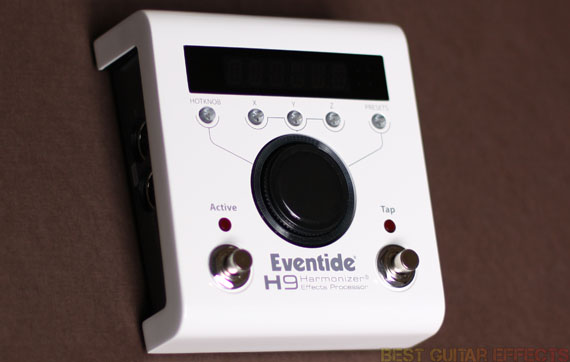
\includegraphics[scale=0.3]{./figuras/eventide-h9.jpg}
					\caption{Foto modelo Eventide H9 - Effects Processor.}
					\label{eventide-h9}
				\end{figure}
				
				\item \textbf{Strymon BigSky}: A empresa Strymon, fundada em meados de 2008, é considerada uma das empresas mais bem sucedidas no universos de pedais de guitarra de linha exclusiva (\textit{boutique-pedals}) que integram algoritmos de tratamento de sinais de áudio extremamente avançados.
				
				Vale salientar que com tantas grandes empresas produzindo diversos produtos, sendo por vezes um réplica do outro, é impressionante ver uma pequena empresa produzir um produto de qualidade notoriamente alta. Foi, de fato, uma reinvenção da roda em termos de qualidade dos efeitos e o resultado esperado pelo usuário final.
				
				\begin{enumerate}
					\item \textbf{Qualidade de Áudio}: \begin{itemize}
						\item Baixo ruído na entrada do dispositivo, alta peformance de aúdio com resolução de 24-bit  e taxa de amostragem de 96kHz, tanto para o conversor Analógico digital quanto para o conversor digital analógico.
						\item 115 db de relação sinal-ruído em 50% de wet mix ou 
					\end{itemize}
					
					\item \textbf{Processador}:
				\end{enumerate}
				
				
				 
			\end{enumerate} 
		
	\subsection{Micontroladores e DSP's}

		O termo sistemas embarcados constituem circuitos eletrônicos que utilizam processadores digitais (microprocessadores ou microcontroladores, etc.) em aplicações dedicadas para determinado equipamento ou produtos.
		
		Os microcontroladores, diferentemente dos microprocessadores, em geral, possuem todos os periféricos necessários num único chip. Seu tamanho também é muito pequeno, mesmo contendo vários periféricos como: memórias, barramentos, \textit{timers}, portas de comunição, conversores de sinal analógicos para digital etc.
		
		Por outro lado, esses dispositivos possuem um desempenho menor que os microprocessadores, mas são ideais em aplicações que necessitam de menores dimensões, tempo e custos.
		
		As linguagens de programação das unidades processadores de sistemas embarcados podem variar, mas em geral, se limitam às linguagens C/C++, \textit{Assembly} e \textit{Java}.
		
		Nessa linha, temos ainda o processador digital de sinais (DSP - \textit{Digital Signal Processing}) e pode definir tanto o processador quanto o processo em si. Esse tipo de tratamento exige um alto desempenho para aplicações numéricas em tempo real.
		
		Os DSP's são construídos para computar de forma eficiente equações de diferenças e algoritmos de transformadas diversas (como a \textit{Fast Fourier Transform} - FFT). As aplicações dos DSP's, em suma, estão relacionadas com sistemas de controle de alta velcodiade, realizações de filtros digitais, transformadas rápidas de \textit{Fourier}, processamento de sons e imagens, entre outras.

	\subsection{Hardwares Comerciais do Efeito \textit{Reverb - Shimmer}}
	
	\subsection{Microcontrolador MSP430F5529 e TMS320}
	
	Foram utilizados ao longo do projeto como soluções de hardware essencialmente o \textit{microntrolador launchpad MSP430F5529}.
	
	Não obstante foram apontados na subseção anterior a respeito das limitações do hardware para tratamento de sinais de áudio em tempo real, o escopo do trabalho levou em consideração a economicidade do hardware em questão, bem como a utilização de operações no domínio do tempo, sem utilização de etapas intermediárias como realização da transformada de \textit{Fourier} para manipulação do sinal de áudio. %melhorar esse texto
	
	Além disso, o projeto teve uma participação do desempenho do TSM320 C2000 o qual, devido ao tempo de aprendizagem do DSP para correta aplicabilidade no projeto, não fora possível. %melhorar o texto


\section{Objetivos e Diagrama de Bloco do Projeto}

	Nosso objetivo neste trabalho é o estudo e a realização de um projeto, desenvolvido em \textit{software} e futuramente aplicado em \textit{hardware}, de um efeito digital de aúdio seletivo em frequência que tem como característica musical a repetição assíncrona do som (reverb) com destaque na utilização de componentes de frequências (harmonicas) na realização desse efeito (\textit{shimmer}).
	
	Nesta parte do trabalho, será mostrado de maneira abstrata os blocos necessários para que obtenha a saída do sistema desejado , ou seja, o efeito do \textit{Reverb} com \textit{Shimmer} implementado em software e executado seja em software ou em hardware.
		
	Temos aqui na figura \ref{bloco-principal} um sinal analógico oriundo e um instrumento musical - guitarra, que passa por um processador de som digital - DSP, o qual procede com todo o trabalho tratamento desse sinal analógico ora convertido amostras digitais. Aplicando, portanto, nesse contexto, um filtro de resposta finita; um algoritmo de seleção de frequências denominado \textit{pitch-shifter} e por fim realimentando o sistema acrescentando um pequeno atraso temporal (\textit{delay}).
	
	\begin{figure}[!h t b]
		\centering
		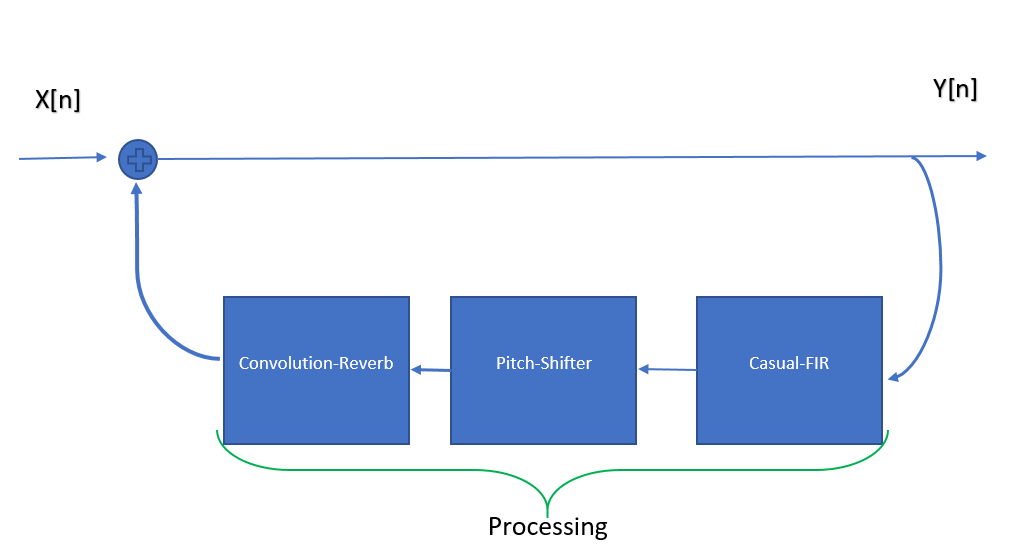
\includegraphics[scale=0.5]{./figuras/diagrama_bloco_principal.PNG}
		\caption{Diagrama de Blocos Principal do Projeto.}
		\label{bloco-principal}
	\end{figure}
	

	Não obstante ao modelo apresentado, também será objeto de estudo os blocos que compõe a conversão do sinal analógico para a realidade de amostras digitais (conversão A/D), bem como o caminho inverso que propõe o envio das amostras a um conversor gerador de níveis de tensão elétrica correspondente (conversão D/A).
	
	
	
	
	

